\documentclass{article}
\usepackage{geometry}
\geometry{a4paper, top=3cm, bottom=3cm, left=2cm, right=2cm}
\usepackage[utf8]{inputenc}
\usepackage[english]{babel}
\usepackage{hyperref}
\makeindex

\title{Advanced Database and Information Systems}
\author{Riccardo Salvalaggio}
\date{19th of April, 2021}

\usepackage{amssymb}
\usepackage{amsmath}
\usepackage{txfonts}
\usepackage{mathdots}
\usepackage[classicReIm]{kpfonts}
\usepackage{graphicx}

% You can include more LaTeX packages here 


\begin{document}

\maketitle
\newpage
\tableofcontents
\newpage

\section{Semi-structured Data models: XML, XPath, XRel}

Structured Data models are obsolete nowadays: inadequate representation, semantic overloading, difficulty on recursion, rigid schema, limited throughput.
Now, semi-unstructured data format: data is no longer dependent on a schema (such as tables), is self-descriptive (good labels), more scalability. This needed is born because data is interlinked between each other (e.g. IoT, smart systems) and generated from DBs.
Anyway, a standardized representation is needed: a new language to structure in a flexible way data and semantically annotate it.

\subsection{XML}

Extensible Markup Language, derived from HTML structure (use of tags), born in late 90s use a tree-structure to describe and organize data.
Start- and end-tag with the inner part of the document are called \textit{element, }the name of it is the name of the tag and the content is the enclosed part. If an element doesn't contain any other tag, the content will be called element text. A tag without content is called empty tag $\mathrm{<}$tag/$\mathrm{>}$.
\begin{center}
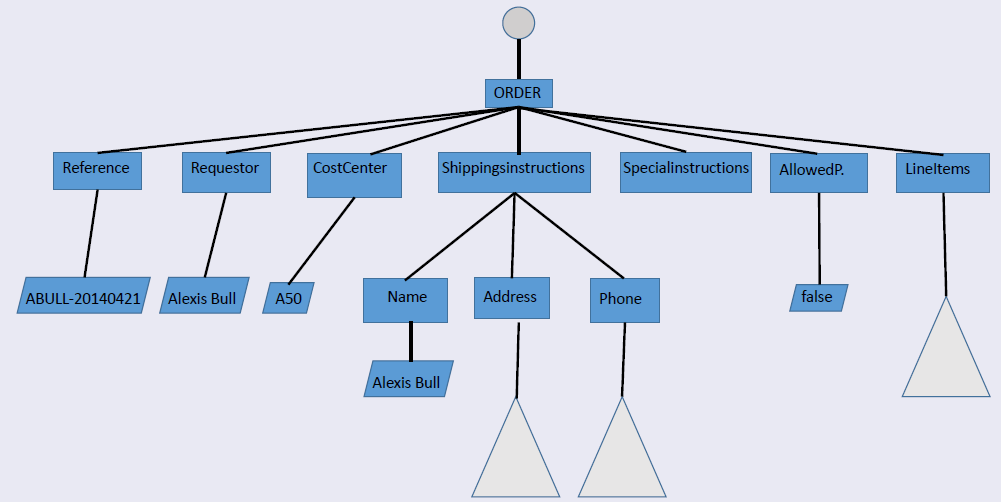
\includegraphics[scale = 0.55]{image1.png}
\end{center}
Tags are ordered, attributes not. An XML-tree is ordered (if depth-first search will reproduce the document order). The textual corresponding representation is called serialization.
It is possible document-recursion (e.g. a message in XML could contain an XML-document) but name conflicts may appear.
Definition of dbis-namespace:\\ $\mathrm{<}$xmlns:dbis=''http://.... ''$\mathrm{>}$\\
\textbf{DTD (Document Type Definition): }define attributes rules of a document (element and attributes types). A document conforms to XML syntax is \textit{well-formed, }if it is also conformed to DTD is \textit{valid.}\\
Definition of element types: \textbf{$\boldsymbol{\mathrm{<}}$!ELEMENT EName Content$\boldsymbol{\mathrm{>}}$}\\
Definition of attribute types: \textbf{$\boldsymbol{\mathrm{<}}$!ATTLIST EName Attr1 AttrType1 {\dots}.}\\
Elements types re global wrt DTD, attributes types are local.\\
\textbf{Element content: }EMPTY, ANY, (\#PCDATA) - ,{\textbar}*+?\\
\textbf{Attribute definition:}\\

\textbf{ Types: }CDATA, (Val1{\textbar}{\dots}{\textbar}Valn), ID, IDREF

\textbf{ Val: }\#REQUIRED, \#IMPLIED, val, \#FIXED val

\subsection{XPath}

XPath is a language to locate subtrees inside an XML-tree by means of location paths (sequence of steps separated by `/'). Each location is formed of an axis, a nodetest and some (opt.) predicates:

\textbf{\textit{Axis::node-test[predicate]}}\\
\begin{center}
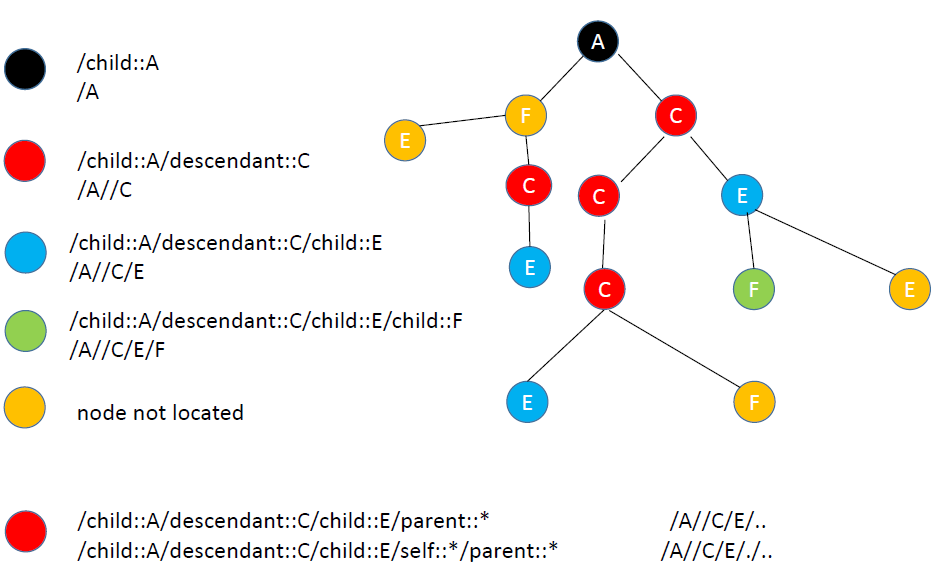
\includegraphics[scale = 0.5]{image2.png}
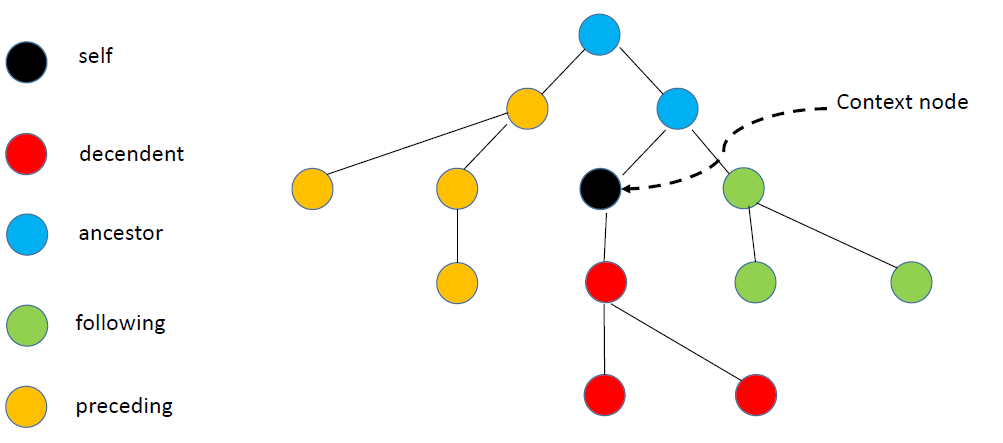
\includegraphics[scale = 0.5]{image3.png}
\end{center}
The path is evaluated relative to a respective context and locates a set of nodes. A context is given by position, size and the node. An absolute location path is the root node.
L${}_{0\ }$= $\mathrm{\{}$r$\mathrm{\}}$ -- root
L${}_{i}$(k) set of nodes determined wrt context node k.
L${}_{i\ }$= U${}_{k\ e\ Li-1}$L${}_{i}$(k).
\textbf{Node-test: }element name, *, text(), node().\\
\textbf{Predicates: }Boolean expression.\\
e.g.: /descendant::*[child::Address]\\
/child::Orders/child::Order[child::CostCenter= "A50"]/child::LineItems.\\
Context is a fact relative to a node set, is composed by: context size (cardinality), context position (its position relative to document order).

\subsection{XRel: How to store XML data physically}
\textbf{Two approaches: }Storing in  column (CLOB - Character Large OBject, type + indexing), Mapping to relational tables (Interval-based, Path-based).\\
XRel: is a Path-Based approach to storage and retrieval of XML documents using
relational databases.
\textbf{Region of an element (node test): }pair of start and end position in the XML doc.\\
\textbf{Region of an attribute: }equal to the parent node plus one.\\
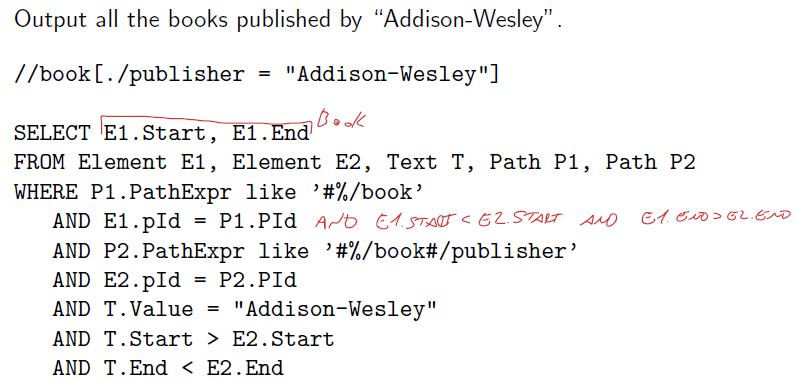
\includegraphics[scale=0.7]{4.png}\\
Use of queries with indexing.

\subsection{XQuery}
The mission of the XML Query project is to provide flexible query facilities to
extract data from real and virtual documents. Collections of XML files will be accessed like DBs.\\
XQuery is a functional language, have a declarative semantics and is strongly typed. An item is an atomic value or a node.\\
Two ways to create element node:\\\\
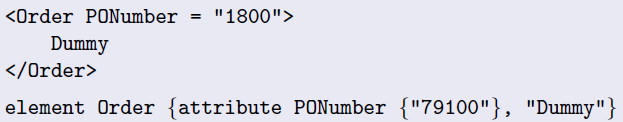
\includegraphics[scale=0.65]{5.png}
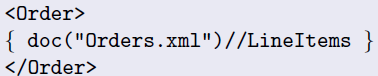
\includegraphics[scale=0.65]{6.png}\\\\
A \textbf{FLWOR-expression} is built out of \textbf{\textit{for-, let-, where-, order- and
return-}}clauses. It evaluates to a stream of tuples, where the tuples are
(variable-name, value) pairs.\\
Two main commands:\\
XMLTable: maps results of an XQuery into relational rows and columns.\\
XMLQuery: return XML-document\\
With XMLTable we refer directly to the path and use passing XMLDoc instruction. With XMLQuery we refer to doc and use RETURNING CONTENT FROM DUAL instruction.\\
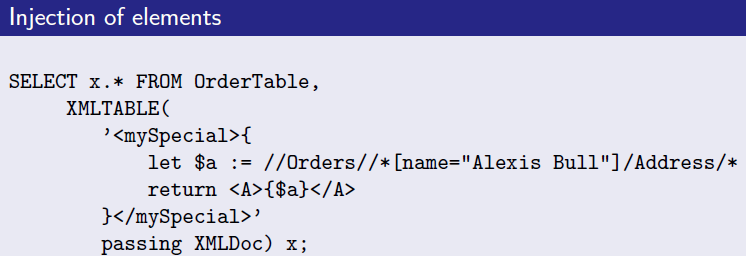
\includegraphics[scale=0.5]{7.png}
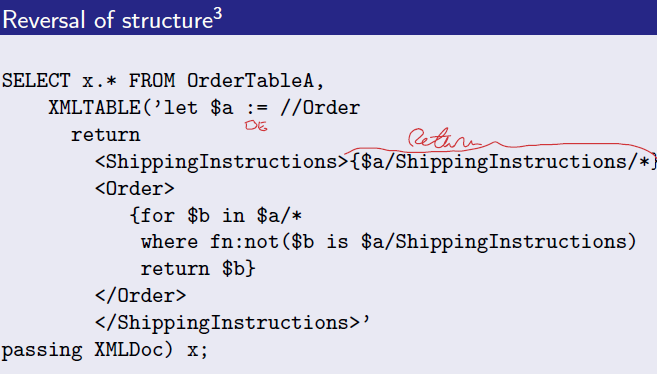
\includegraphics[scale=0.5]{8.png}\\
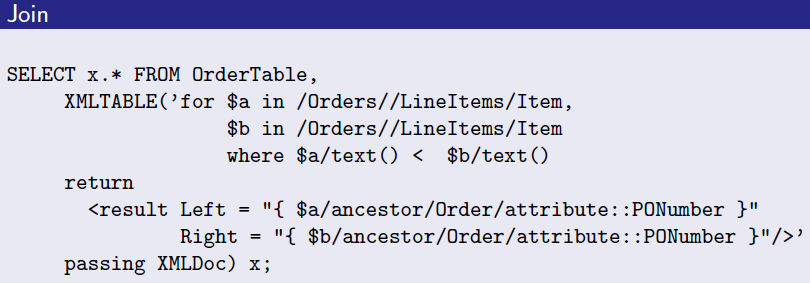
\includegraphics[scale=0.5]{9.png}\\
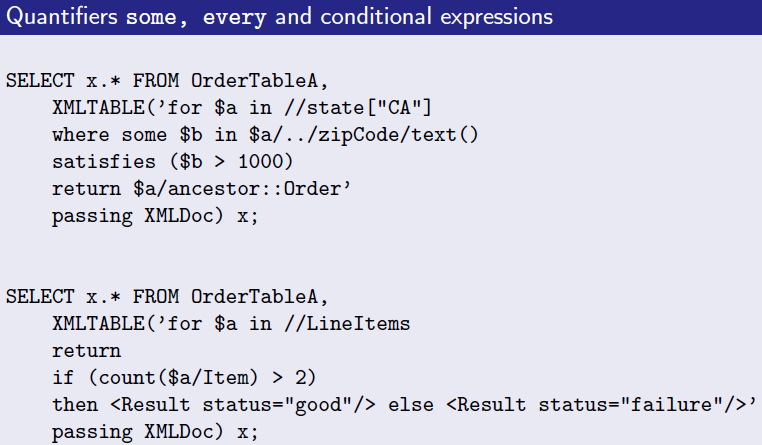
\includegraphics[scale=0.5]{10.png}
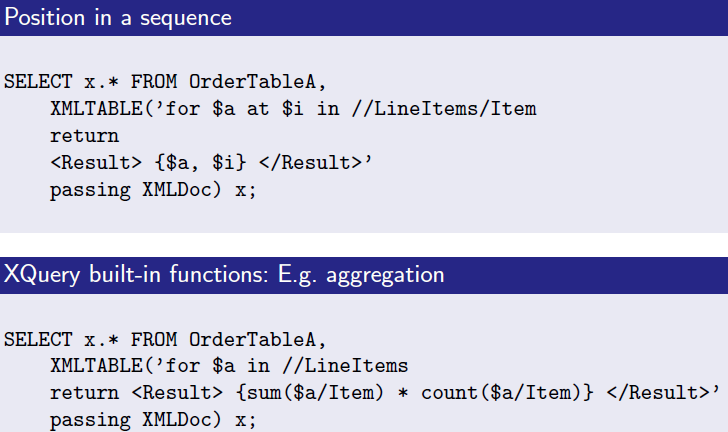
\includegraphics[scale=0.5]{11.png}\\
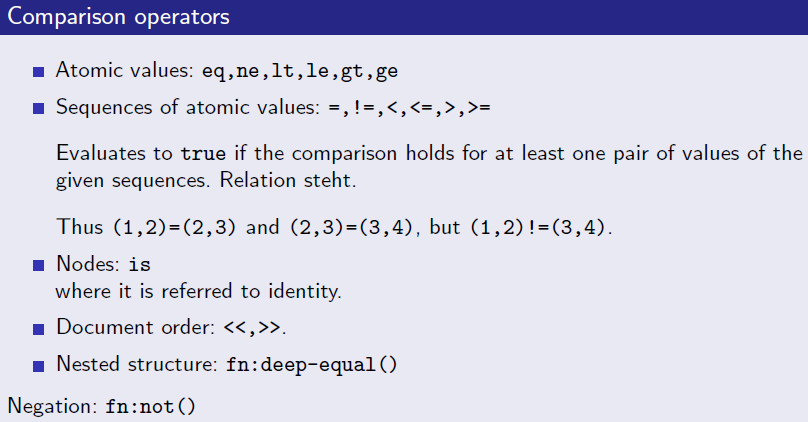
\includegraphics[scale=0.5]{12.png}\\

\section{JSON and MONGODB}

\subsection{JSON (JavaScript Object Notation)}
It is a very lightweight data exchange format based on JavaScript used for data exchange over Web.\\
It is based on two basic constructs:\\
\textbf{1. Array: }comma-separated list of things enclosed by brackets.\\
\textbf{2. Object: }comma-separated set of pairs enclosed by braces.\\\\
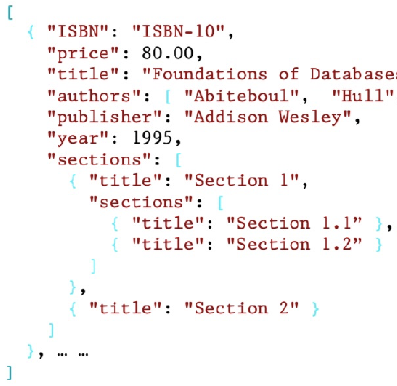
\includegraphics[scale=0.5]{18.png}\\

\subsection{MongoDB}
Document database designed for ease of development and scaling.\\
NoSQL database types:\\
\textbf{1. Key-value stores}\\
\textbf{2. Document databases:} data structure.\\
\textbf{3. Wide-column stores:} store columns of data.\\
\textbf{4. Graph stores:} store info about networks.\\
Uses JSON (BSON). MongoDB stores data records as BSON documents. BSON is a binary representation of JSON documents.\\\\
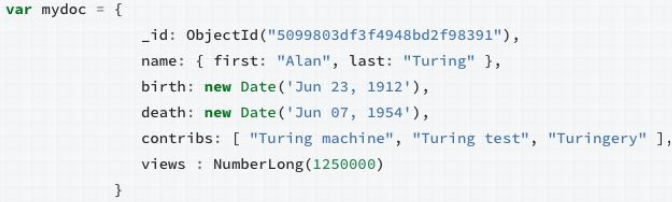
\includegraphics[scale=0.5]{19.png}\\\\
- Database = a number of collections.\\
- Collection = a list of documents.\\
- Each document stored in a collection requires a unique $\_$id
field that acts as a primary key.\\
CRUD operations: Create, Read, Update, Delete.\\
Insert commands: .insertOne(), .insertMany().\\

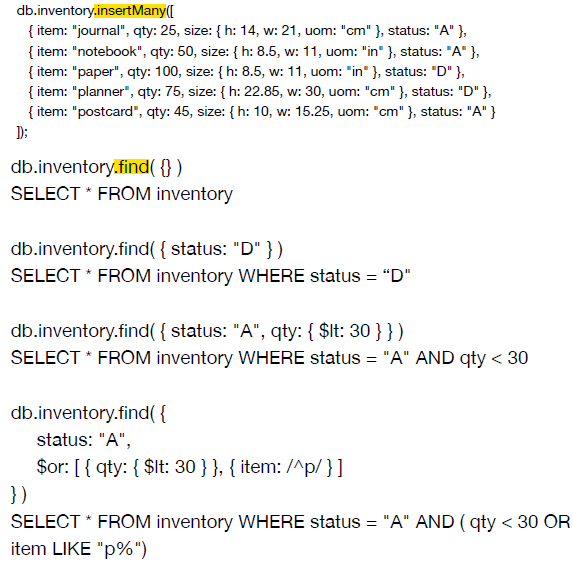
\includegraphics[scale=0.5]{20.png}
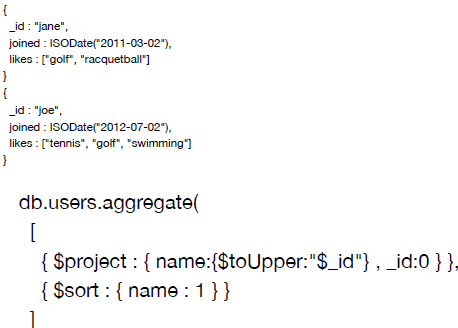
\includegraphics[scale=0.5]{21.png}\\

\begin{figure}[h!]
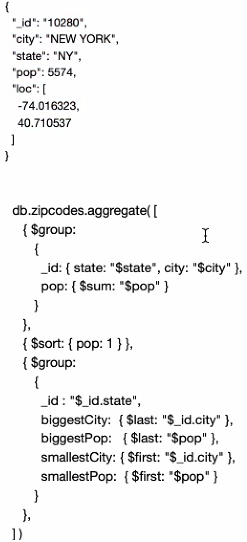
\includegraphics[scale=0.7]{13.png}
\caption{Largest and smallest cities by state.}
\end{figure}
\begin{figure}[h!]
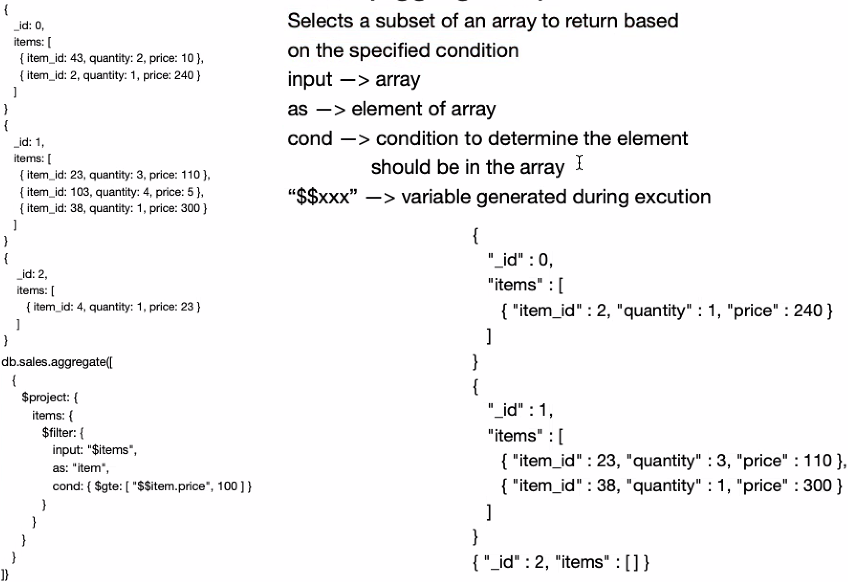
\includegraphics[scale=0.7]{14.png}
\caption{filter.}
\end{figure}

\begin{figure}[h!]
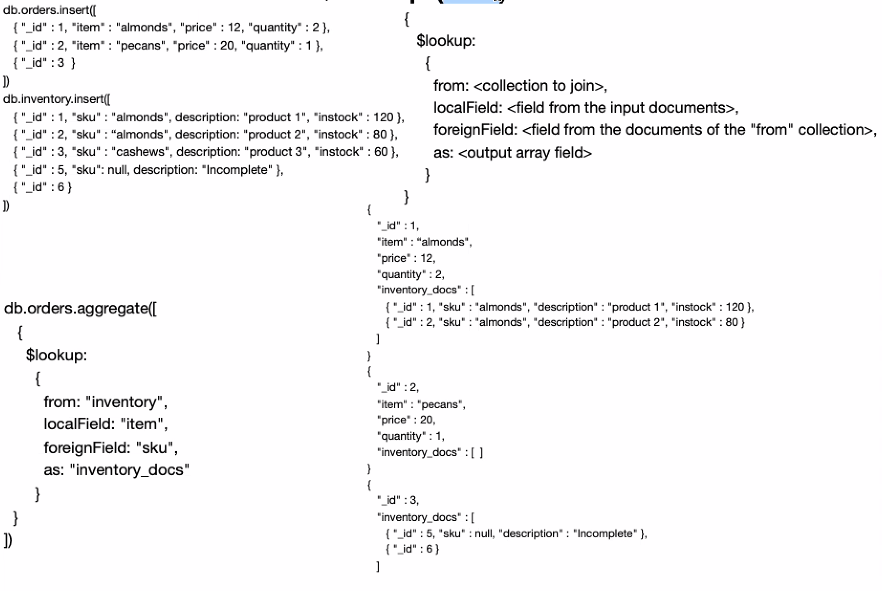
\includegraphics[scale=0.7]{15.png}
\caption{lookup(join).}
\end{figure}
\begin{figure}[h!]
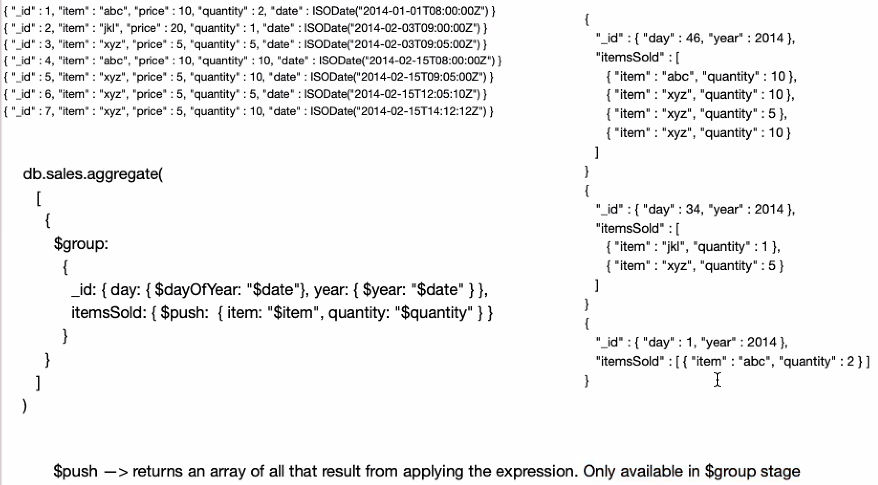
\includegraphics[scale=0.7]{16.png}
\caption{push.}
\end{figure}
\begin{figure}[t]
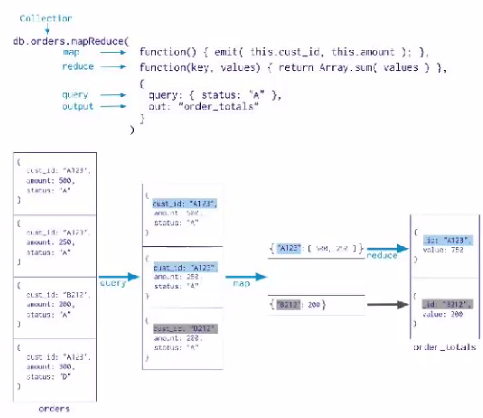
\includegraphics[scale=0.7]{17.png}
\caption{Map-reduce:Used to condense large volumes of data and emits key-value pairs. For keys with multiple values, MONGODB applies the reduce phase and then stores results in a collection.}
\end{figure}


\end{document}




